% fig_pott_logic.tex
% TR-33: POTT scheme logic diagram — End A (local) and End B (remote)
%
% Shows the two-terminal logic:
%   End A: Z2_local asserts → waits for permissive from B
%   End B: 67Q/87L asserts (forward) → sends permissive carrier to A
%   Trip at A: Z2_A AND perm_rx AND memory_valid
%
% Layout: horizontal, End A left, End B right, carrier arrows crossing

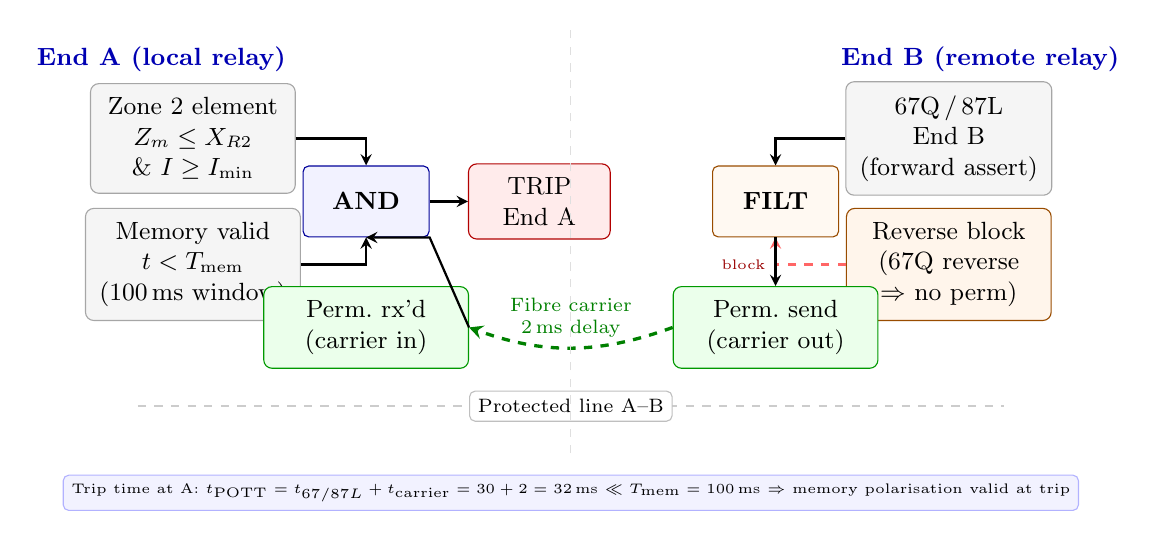
\begin{tikzpicture}[
  every node/.style = {font=\small},
  blk/.style        = {draw=gray!70, fill=gray!8, rounded corners=3pt,
                        inner sep=5pt, align=center, minimum width=2.6cm,
                        minimum height=0.9cm},
  gate/.style       = {draw=blue!60!black, fill=blue!5, rounded corners=2pt,
                        inner sep=4pt, align=center, minimum width=1.6cm,
                        minimum height=0.9cm, font=\small\bfseries},
  trip/.style       = {draw=red!70!black, fill=red!8, rounded corners=3pt,
                        inner sep=5pt, align=center, minimum width=1.8cm,
                        minimum height=0.9cm},
  arr/.style        = {->, >=stealth, thick},
  carr/.style       = {->, >=stealth, very thick, green!50!black,
                        dashed, bend left=15},
]

% ── END A (left side) ─────────────────────────────────────────────────────────
\node[blk] (Z2A) at (-4.8, 1.2) {Zone~2 element\\$Z_m \leq X_{R2}$\\\& $I \geq I_\mathrm{min}$};
\node[blk] (memA) at (-4.8, -0.4) {Memory valid\\$t < T_\mathrm{mem}$\\(100\,ms window)};

% AND gate End A
\node[gate] (andA) at (-2.6, 0.4) {AND};

% Perm receive block
\node[blk, fill=green!8, draw=green!60!black] (permRx) at (-2.6, -1.2)
  {Perm.\ rx'd\\(carrier in)};

% Trip output
\node[trip] (tripA) at (-0.4, 0.4) {TRIP\\End A};

% ── END B (right side) ────────────────────────────────────────────────────────
\node[blk] (B67) at (4.8, 1.2) {67Q\,/\,87L\\End B\\(forward assert)};
\node[blk, fill=orange!8, draw=orange!60!black] (BrevBlk) at (4.8, -0.4)
  {Reverse block\\(67Q reverse\\$\Rightarrow$ no perm)};

% OR/select gate End B
\node[gate, fill=orange!5, draw=orange!60!black] (selB) at (2.6, 0.4)
  {FILT};

% Perm send block
\node[blk, fill=green!8, draw=green!60!black] (permTx) at (2.6, -1.2)
  {Perm.\ send\\(carrier out)};

% ── CONNECTIONS End A ─────────────────────────────────────────────────────────
\draw[arr] (Z2A.east)    -| (andA.north);
\draw[arr] (memA.east)   -| (andA.south);
\draw[arr] (permRx.east) -- (andA.south east) |- (andA.south);
\draw[arr, thick] (andA.east) -- (tripA.west);

% ── CONNECTIONS End B ─────────────────────────────────────────────────────────
\draw[arr] (B67.west)      -| (selB.north);
\draw[arr, dashed, red!60] (BrevBlk.west) -| (selB.south)
  node[midway, left, font=\tiny, red!60!black] {block};
\draw[arr] (selB.south) -- (permTx.north);

% ── CARRIER (B → A) ──────────────────────────────────────────────────────────
\draw[carr] (permTx.west) to[bend left=20]
  node[above, midway, font=\scriptsize, green!50!black,
       align=center] {Fibre carrier\\2\,ms delay}
  (permRx.east);

% ── PROTECTED LINE label ──────────────────────────────────────────────────────
\draw[gray!50, very thick] (-0.0, -2.2) -- (0.0, -2.2);
\draw[gray!40, thick, dashed] (-5.5, -2.2) -- (5.5, -2.2);
\node[draw=gray!50, fill=white, rounded corners=2pt,
      font=\scriptsize, inner sep=3pt] at (0, -2.2)
  {Protected line A--B};

% ── BUS labels ────────────────────────────────────────────────────────────────
\node[font=\small\bfseries, blue!70!black] at (-5.2, 2.2) {End A (local relay)};
\node[font=\small\bfseries, blue!70!black] at ( 5.2, 2.2) {End B (remote relay)};

% ── Divider ──────────────────────────────────────────────────────────────────
\draw[gray!25, dashed] (0, -2.8) -- (0, 2.6);

% ── Timing annotation ────────────────────────────────────────────────────────
\node[draw=blue!30, fill=blue!5, rounded corners=2pt,
      font=\tiny, inner sep=3pt, align=center]
  at (0, -3.3)
  {Trip time at A: $t_\mathrm{POTT} = t_{67/87L} + t_\mathrm{carrier} = 30 + 2 = 32$\,ms
   $\ll T_\mathrm{mem} = 100$\,ms $\Rightarrow$ memory polarisation valid at trip};

\end{tikzpicture}
